\section{System overview}

Heart of SoC is CPU. The CPU is only one master on the system bus and it control
all communication on this bus. To the CPU is directly connected interrupt
controller.

Bus consist of 24b address, 32b MOSI data, 32b MISO data, clock, reset, write,
read and ack signals. There is also 16b bus for interrupts.

All the peripherals are connected to the system bus, CPU select peripheral to
communicate with through address. Peripheral control ack signal to say to CPU
"data is ready for read" when CPU want read data, or "data is written" when CPU
want write data. This allow slower peripheral to cooperate with CPU, CPU simply
wait for them.

Some peripherals have special pins, these are commonly connected to the top
level entity pins, but there are few that are connected internally, for example
pll outputs.

SoC have multiple clock domain. There are four clock domains, one is 
for VGA driver ($31,5 MHz$), second if for UART baudrate generator 
($38,4 MHz$), third is for SDRAM driver ($100 MHz$) and last is for 
rest of SoC including CPU ($50 MHz$). Clocks are generated by pll from 
single $50 MHz$ input. $50 MHz$ was selected because $50 MHz$ 
oscillators are common on the Terasic FPGA boards.

\begin{wrapfigure}{L}{0.6\textwidth}
    \centering
    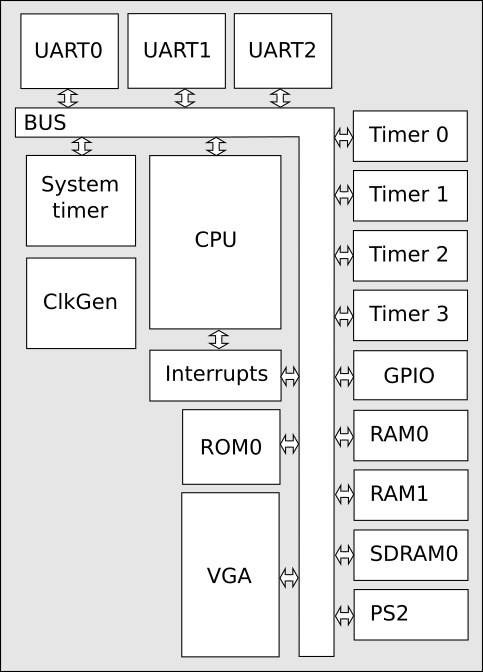
\includegraphics[width=0.55\textwidth]{img/MARK_II.png}
    \caption{MARK-II system architecture}
    \label{fig:sysarch}
\end{wrapfigure}

On the figure \ref{fig:sysarch} is simple high level schematic of MARK-II
system architecture, you can see bus, CPU and all units. Clkgen is only one unit
that isn't connected to the main BUS. It isn't need any configuration.

Another special module is interrupt control unit. It is connected directly to
the CPU and also connected on system BUS. Interrupt control unit have interrupt
sources that are connected to the others modules such are Timers or UARTs.
